% This is LLNCS.DEM the demonstration file of
% the LaTeX macro package from Springer-Verlag
% for Lecture Notes in Computer Science,
% version 2.4 for LaTeX2e as of 16. April 2010
%
\documentclass{llncs}
%
\usepackage{makeidx}  % allows for indexgeneration
%
\usepackage{graphicx}
\usepackage{mathtools}

\DeclareMathOperator*{\argmin}{argmin}

\begin{document}
%
\frontmatter          % for the preliminaries
%
\pagestyle{headings}  % switches on printing of running heads


%

%
\mainmatter              % start of the contributions
%
\title{Yelp Recommendation System Based on Collaborative Filtering}
%
\titlerunning{Yelp Recommendation System Based on Collaborative Filterings}  % abbreviated title (for running head)
%                                     also used for the TOC unless
%                                     \toctitle is used
%
\author{Sainan He, Jiaoyang Fu, Yameng Li}
%
\authorrunning{Ivar Ekeland et al.} % abbreviated author list (for running head)
%
%%%% list of authors for the TOC (use if author list has to be modified)
\tocauthor{Sainan He, Jiaoyang Fu, Yameng Li}
%
\institute{Electrical and Computer Engineering, University of Waterloo, Canada,\\
\email{{s66he, j45fu, y949li}@uwaterloo.cau}
}

\maketitle              % typeset the title of the contribution

\begin{abstract}
Based on Yelp Data Challenge dataset, we aim to develop a predictive personalized recommendation system on user’s review star rating for restaurants, applying collaborative filtering algorithms. In particular, we implement and compare the performances of four algorithms including baseline, User-based and Item-based collaborative filtering and Singular Value Decomposition (SVD). We evaluate our results by comparing our predicted rating to the actual rating using Root Mean Squared Error(RMSE) and Mean Absolute Error(MAE) metrics
\keywords{Recommendation System, Collaborative filtering, Yelp Data Challenge}
\end{abstract}
%
\section{Introduction}
%
With rapid development of advanced technology, people nowadays can achieve the things that they desired faster and more effectively than ever. While, at the same time, the requirements for accurate, personalized and convenient services are increasing. Fortunately, Yelp contributes to providing reasonable recommendations of various businesses to users, e.g., restaurants.

Yelp collected review dataset which records how well each user rates for limited amount of restaurants. Based on these review history, it suggests favored restaurants to users. The problem is that Yelp seems to offer similar recommendations that are popular for various users. In fact, people may have diverse preferences to food. For instance, some users may prefer Asian food, while others may favor Mexican food. In fact, yelp did not consider these factors too much. Therefore, it seems still have some room to improve the recommendation system in the personalization aspect.

Collaborative filtering, a method making predictions based on a large dataset used by some recommendation system like Yelp, Amazon, and Netflix. It automatically predict about the interests of a user by collecting preference or tastes information from other users. Furthermore, there are numerous collaborative filtering methods, such as baseline, K- nearest neighbor, and matrix decomposition. This paper aims to compare how accurate each methods applying on Yelp Data Challenge through using Root metric Mean Squared Error(RMSE) and Mean Absolute Error(MAE).

\section{Literature Review}
There are generally three types of recommendation systems: content-based filtering, collaborative filtering and hybrid approaches. Content-based recommendation systems work with users’ profile and items’ characteristics. The feature used to build profiles are often a set of keywords. For example, a music recommendation system\cite{MJ} implemented with content-based filtering, each song is assigned an attribute manually. If a user’s profile shows interests in songs with particular attributes, similar songs will be recommended to the user. The limitations of these systems is that it always recommends similar items to user that he has already purchased and it’s difficult to recommend items for new users. 

Collaborative filtering try to predict the utility of items for a particular user based on the items previously rated by other users with similar tastes and preferences. In\cite{Bruno} the author builds a recommendation system for a retail store using three kinds of collaborative filtering algorithms - memory based approach, matrix factorization and bigram matrix method. Collaborative filtering also has limitations that it is difficult to recommend items for new users, to recommend items which have not been rated before, and to recommend when rating information is insufficient. 

Hybrid approach combines multiple techniques to overcome the limitations of individual systems. A restaurant recommendation system for yelp user\cite{Sumedh} adopts hybrid approach by extracting collaborative and content-based features to identify customer and restaurant profiles. A hybrid cascade of K-nearest neighbor clustering, weighted bi-partite graph projection, and several other learning algorithms are proposed. 

\section{Data}
We collect our data from Yelp recommendation Kaggle competition\cite{yelp},This dataset contains 11,537 businesses, 8282 check-in sets, 43873 users, and 229907 reviews. Each user has a unique user id as well as business. We target “Restaurant” in the city of “Phoenix” as it is more reasonable to recommend restaurants for users in the same city and Phoenix has the most amount of review records among all the cities.
\subsection{ Data Processing}
The original data file is in json format. We firstly parse the raw data of information from users, businesses and reviews, respectively and merge them into one dataframe. Then we extract the records with features of “Restaurants” and “Phoenix” for further analysis. After this approach, we have 17145 users, 1454 business and 52749 reviews.

Because many users only review a few restaurants, our dataset yields a sparsity of 99.79\% which can be visualized from figure 1. To solve this problem, we create a smaller dataset which only consider  restaurants reviewed by more than 50 users.
%

\begin{figure}
	\begin{minipage}[t]{0.5\textwidth}
		\centering
		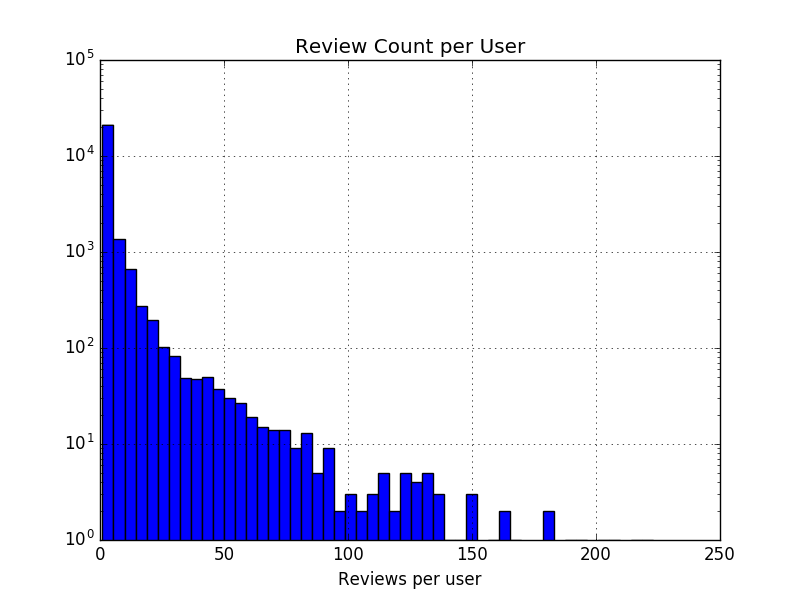
\includegraphics[width=2.2in]{fig1.png}
		\caption{User review count}
		\label{fig:side:a}
	\end{minipage}%
	\begin{minipage}[t]{0.5\textwidth}
		\centering
		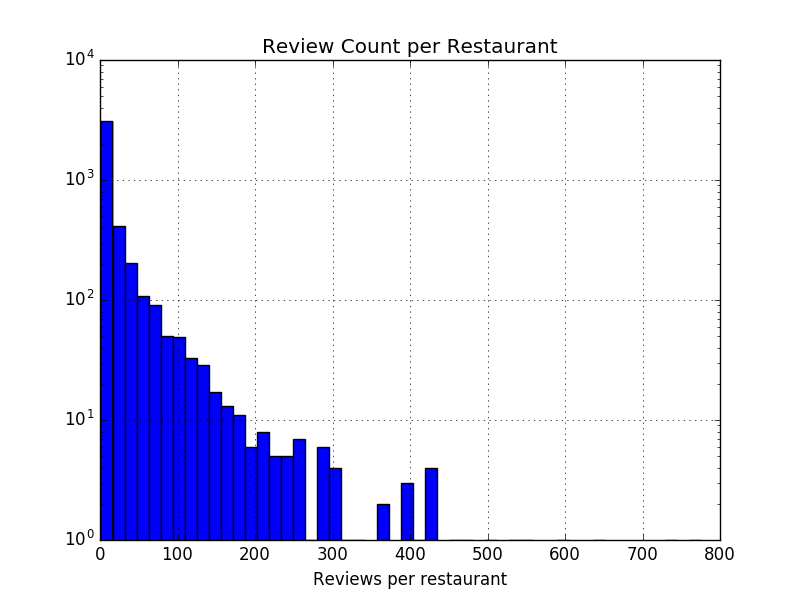
\includegraphics[width=2.2in]{fig2.png}
		\caption{Restaurants review count}
		\label{fig:side:b}
	\end{minipage}
\end{figure}

\subsection{Training and Testing Sets}
%
In order to evaluate the performance of our recommendation system, we divided our data into training and testing datasets. We extract a list of all restaurants each user has rated, take 80\% of this list as training set and 20\% as test set. 

\section{Methods}
\subsection{Baseline}
Our baseline model is similar to the model implemented by\cite{Yehuda} which is a mean predictor and accounts for the user and item effects. 
\begin{equation}
\ b_{ur} = \mu + b_u + b_r \ .
\end{equation}

Here $\mu$ is the mean rating of reviews of all business by all users. The parameter $b_u$ indicates the difference between the average rating of user $u$ and $\mu$. The parameter $b_i$ indicates the difference between the average rating of business $i$ and $\mu$. This will normalize the widely noticed tendency of some user giving higher rating than others and some restaurants getting higher ratings than others.


\subsection{User-based Collaborative Filtering}

\subsection{User-based Collaborative Filtering}

\subsection{Singular Value Decomposition}
Singular Value Decomposition(SVD) is a latent factor method which popularly applied in Netflix Prize competition. A matrix can be approximated with SVD by multiplying two generated feature matrices $P$ and $Q$ with rank $k$.
\begin{equation}
\hat{R_{ij}} = P_iQ_{j}^{T}
\end{equation}
In this paper, the matrix $R$ is a ratings matrix with rows representing all the users, and columns representing businesses. For example $R_{ij}$ represents the rating from user $i$ to restaurant $j$. Then, minimizing the squared differences between the rating matrix $R$ and the SVD approximated matrix $\hat{R}$. Thus,projecting user and restaurants rating matrix into two lower dimension feature matrices $P$ as user feature matrix and $Q$ as restaurant matrix. In order to improve the SVD prediction accuracy, subtract the global average rating, $\mu$.

\begin{equation}
\hat{R_{ij}} = P_iQ_{j}^{T} + \mu
\end{equation}

\begin{equation}
\argmin_{P,Q}\sum_{(i,j)\in{R}}{(R_{ij} - \mu - P_iQ_{j}^{T})}^2
\end{equation}

We also add a regularization to avoid overfitting to our training set.

\begin{equation}
\argmin_{P,Q}\sum_{(i,j)\in{R}}{(R_{ij} - \mu - P_iQ_{j}^{T})}^2 + \lambda({\left\|P_i\right\|}^2 + {\left\|Q_j\right\|}^2 )
\end{equation}

In order to find optimum matrices for $P$ and $Q$, we implement the alternating least squares method as described by Cichocki and Zhou\cite{abc},\cite{zhou}.

After obtaining the predicted rating by matrices $P$ and $Q$ via SVD, add the global mean back to each predicted rating. We take $k$ as 20 and $\lambda$ as 0.01.


\section{Experiments and Results}
%
\subsection{Evaluation Metrics}
Our goal is to predict the rating a user would give to a restaurant. We predict the rating that user has not rated in the training dataset, but the true rating is stored in the test dataset. We use the root-mean-square error and mean-absolute error for evaluation.
\begin{equation}
\ RMSE = \sqrt{\frac{\sum{\left(r'_{u,i} - r_{u,i}\right)}^2}{N}}
\end{equation}
\begin{equation}
\ MAE = \sqrt{\frac{\sum{\left|r'_{u,i} - r_{u,i}\right|}}{N}}
\end{equation}

Here $r_{u,i}$ is the predicted rating from user $u$ on item $i$ and $r'_{u,i}$ is the true rating; $N$ is the size of test dataset. 
\section{Implementation}
Our work was implemented by Python. We used Pandas for data processing which is an open source, data analysis library. The original json files were loaded into three dataframe storing information of users, business and reviews respectively. We joined the business and reviews dataframes based on business id and then joined with users dataframe on user id. After parsing the raw data, we used the key “Category” and “City” to extract records of “Restaurants” and “Phoenix”. As to reboost spasity problem, we computed the count of reviews grouped by restaurant id and filtered the restaurants getting rid of the restaurants which have fewer than 50 reviews. 

After re-organizing the data, we used dictionay data structure to built the user-item matrix. For each records in the joined dataframe, we extract user as the key, the value of each key is a nested dictionary with business id as key and review rating as value, e.g. $\{user\_id: \{restautant\_id: rating\}\}$. Meanwhile, we also built another item-user matrix which can be indexed by restaurant id, e.g. $\{restautant\_id: \{user\_id: rating\}\}$.


\section{Results}
The performance of our baseline predictor is $RMSE = $, $MAE= $.




%
% ---- Bibliography ----
%
\begin{thebibliography}{}
%
\bibitem {MJ}
MJ Pazzani, D Billsus.:
Content-based Recommendation Systems. In The adaptive web, pp. 325–341. Springer (1981) 

\bibitem {Bruno}
Bruno Pradel, Savaneary Sean, Julien Delporte.: 
A Case Study in a Recommender System Based on Purchase Data. Proceedings of the 17th ACM SIGKDD international conference on Knowledge discovery and data mining, pp. 377-385 (2011)

\bibitem {Sumedh}
Sumedh Sawant, Gina Pai.:
Yelp Food Recommendation System

\bibitem {yelp}
https://www.kaggle.com/c/yelp-recsys-2013

\bibitem {Yehuda}
Yehuda Koren.: 
Factorization meets the neighborhood: a multifaceted collaborative filtering model. In Proceedings of the 14th ACM SIGKDD international conference on Knowledge discovery and data mining (KDD '08), pp. 426-434 (2008)

\bibitem {abc}
Andrzej Cichocki, Rafal Zdunek:. Regularizaed Alternating Least Squares Algorithms for Non-negative Matrix/Tensor Factorization. pp. 793-802 (2007)

\bibitem {zhou}
Yunhong Zhou, Dennis Wikinson, Robert Schreiber, and Rong Pan.: Large-Scale Parallel Collaborative Filtering for the Netflix Prize (2008)

\end{thebibliography}

%
% second contribution with nearly identical text,
% slightly changed contribution head (all entries
% appear as defaults), and modified bibliography
%
\title{Hamiltonian Mechanics2}

\author{Ivar Ekeland\inst{1} \and Roger Temam\inst{2}}

\institute{Princeton University, Princeton NJ 08544, USA
\and
Universit\'{e} de Paris-Sud,
Laboratoire d'Analyse Num\'{e}rique, B\^{a}timent 425,\\
F-91405 Orsay Cedex, France}

\maketitle
%
% Modify the bibliography environment to call for the author-year
% system. This is done normally with the citeauthoryear option
% for a particular contribution.
\makeatletter
\renewenvironment{thebibliography}[1]
     {\section*{\refname}
      \small
      \list{}%
           {\settowidth\labelwidth{}%
            \leftmargin\parindent
            \itemindent=-\parindent
            \labelsep=\z@
            \if@openbib
              \advance\leftmargin\bibindent
              \itemindent -\bibindent
              \listparindent \itemindent
              \parsep \z@
            \fi
            \usecounter{enumiv}%
            \let\p@enumiv\@empty
            \renewcommand\theenumiv{}}%
      \if@openbib
        \renewcommand\newblock{\par}%
      \else
        \renewcommand\newblock{\hskip .11em \@plus.33em \@minus.07em}%
      \fi
      \sloppy\clubpenalty4000\widowpenalty4000%
      \sfcode`\.=\@m}
     {\def\@noitemerr
       {\@latex@warning{Empty `thebibliography' environment}}%
      \endlist}
      \def\@cite#1{#1}%
      \def\@lbibitem[#1]#2{\item[]\if@filesw
        {\def\protect##1{\string ##1\space}\immediate
      \write\@auxout{\string\bibcite{#2}{#1}}}\fi\ignorespaces}
\makeatother
%
\begin{abstract}
The abstract should summarize the contents of the paper
using at least 70 and at most 150 words. It will be set in 9-point
font size and be inset 1.0 cm from the right and left margins.
There will be two blank lines before and after the Abstract. \dots
\keywords{graph transformations, convex geometry, lattice computations,
convex polygons, triangulations, discrete geometry}
\end{abstract}
%
\section{Fixed-Period Problems: The Sublinear Case}
%
With this chapter, the preliminaries are over, and we begin the search
for periodic solutions to Hamiltonian systems. All this will be done in
the convex case; that is, we shall study the boundary-value problem
\begin{eqnarray*}
  \dot{x}&=&JH' (t,x)\\
  x(0) &=& x(T)
\end{eqnarray*}
with $H(t,\cdot)$ a convex function of $x$, going to $+\infty$ when
$\left\|x\right\| \to \infty$.

%
\subsection{Autonomous Systems}
%
In this section, we will consider the case when the Hamiltonian $H(x)$
is autonomous. For the sake of simplicity, we shall also assume that it
is $C^{1}$.

We shall first consider the question of nontriviality, within the
general framework of
$\left(A_{\infty},B_{\infty}\right)$-subquadratic Hamiltonians. In
the second subsection, we shall look into the special case when $H$ is
$\left(0,b_{\infty}\right)$-subquadratic,
and we shall try to derive additional information.
%
\subsubsection{The General Case: Nontriviality.}
%
We assume that $H$ is
$\left(A_{\infty},B_{\infty}\right)$-sub\-qua\-dra\-tic at infinity,
for some constant symmetric matrices $A_{\infty}$ and $B_{\infty}$,
with $B_{\infty}-A_{\infty}$ positive definite. Set:
\begin{eqnarray}
\gamma :&=&{\rm smallest\ eigenvalue\ of}\ \ B_{\infty} - A_{\infty} \\
  \lambda : &=& {\rm largest\ negative\ eigenvalue\ of}\ \
  J \frac{d}{dt} +A_{\infty}\ .
\end{eqnarray}

Theorem 21 tells us that if $\lambda +\gamma < 0$, the boundary-value
problem:
\begin{equation}
\begin{array}{rcl}
  \dot{x}&=&JH' (x)\\
  x(0)&=&x (T)
\end{array}
\end{equation}
has at least one solution
$\overline{x}$, which is found by minimizing the dual
action functional:
\begin{equation}
  \psi (u) = \int_{o}^{T} \left[\frac{1}{2}
  \left(\Lambda_{o}^{-1} u,u\right) + N^{\ast} (-u)\right] dt
\end{equation}
on the range of $\Lambda$, which is a subspace $R (\Lambda)_{L}^{2}$
with finite codimension. Here
\begin{equation}
  N(x) := H(x) - \frac{1}{2} \left(A_{\infty} x,x\right)
\end{equation}
is a convex function, and
\begin{equation}
  N(x) \le \frac{1}{2}
  \left(\left(B_{\infty} - A_{\infty}\right) x,x\right)
  + c\ \ \ \forall x\ .
\end{equation}

%
\begin{proposition}
Assume $H'(0)=0$ and $ H(0)=0$. Set:
\begin{equation}
  \delta := \liminf_{x\to 0} 2 N (x) \left\|x\right\|^{-2}\ .
  \label{2eq:one}
\end{equation}

If $\gamma < - \lambda < \delta$,
the solution $\overline{u}$ is non-zero:
\begin{equation}
  \overline{x} (t) \ne 0\ \ \ \forall t\ .
\end{equation}
\end{proposition}
%
\begin{proof}
Condition (\ref{2eq:one}) means that, for every
$\delta ' > \delta$, there is some $\varepsilon > 0$ such that
\begin{equation}
  \left\|x\right\| \le \varepsilon \Rightarrow N (x) \le
  \frac{\delta '}{2} \left\|x\right\|^{2}\ .
\end{equation}

It is an exercise in convex analysis, into which we shall not go, to
show that this implies that there is an $\eta > 0$ such that
\begin{equation}
  f\left\|x\right\| \le \eta
  \Rightarrow N^{\ast} (y) \le \frac{1}{2\delta '}
  \left\|y\right\|^{2}\ .
  \label{2eq:two}
\end{equation}

\begin{figure}
\vspace{2.5cm}
\caption{This is the caption of the figure displaying a white eagle and
a white horse on a snow field}
\end{figure}

Since $u_{1}$ is a smooth function, we will have
$\left\|hu_{1}\right\|_\infty \le \eta$
for $h$ small enough, and inequality (\ref{2eq:two}) will hold,
yielding thereby:
\begin{equation}
  \psi (hu_{1}) \le \frac{h^{2}}{2}
  \frac{1}{\lambda} \left\|u_{1} \right\|_{2}^{2} + \frac{h^{2}}{2}
  \frac{1}{\delta '} \left\|u_{1}\right\|^{2}\ .
\end{equation}

If we choose $\delta '$ close enough to $\delta$, the quantity
$\left(\frac{1}{\lambda} + \frac{1}{\delta '}\right)$
will be negative, and we end up with
\begin{equation}
  \psi (hu_{1}) < 0\ \ \ \ \ {\rm for}\ \ h\ne 0\ \ {\rm small}\ .
\end{equation}

On the other hand, we check directly that $\psi (0) = 0$. This shows
that 0 cannot be a minimizer of $\psi$, not even a local one.
So $\overline{u} \ne 0$ and
$\overline{u} \ne \Lambda_{o}^{-1} (0) = 0$. \qed
\end{proof}
%
\begin{corollary}
Assume $H$ is $C^{2}$ and
$\left(a_{\infty},b_{\infty}\right)$-subquadratic at infinity. Let
$\xi_{1},\allowbreak\dots,\allowbreak\xi_{N}$  be the
equilibria, that is, the solutions of $H' (\xi ) = 0$.
Denote by $\omega_{k}$
the smallest eigenvalue of $H'' \left(\xi_{k}\right)$, and set:
\begin{equation}
  \omega : = {\rm Min\,} \left\{\omega_{1},\dots,\omega_{k}\right\}\ .
\end{equation}
If:
\begin{equation}
  \frac{T}{2\pi} b_{\infty} <
  - E \left[- \frac{T}{2\pi}a_{\infty}\right] <
  \frac{T}{2\pi}\omega
  \label{2eq:three}
\end{equation}
then minimization of $\psi$ yields a non-constant $T$-periodic solution
$\overline{x}$.
\end{corollary}
%

We recall once more that by the integer part $E [\alpha ]$ of
$\alpha \in \bbbr$, we mean the $a\in \bbbz$
such that $a< \alpha \le a+1$. For instance,
if we take $a_{\infty} = 0$, Corollary 2 tells
us that $\overline{x}$ exists and is
non-constant provided that:

\begin{equation}
  \frac{T}{2\pi} b_{\infty} < 1 < \frac{T}{2\pi}
\end{equation}
or
\begin{equation}
  T\in \left(\frac{2\pi}{\omega},\frac{2\pi}{b_{\infty}}\right)\ .
  \label{2eq:four}
\end{equation}

%
\begin{proof}
The spectrum of $\Lambda$ is $\frac{2\pi}{T} \bbbz +a_{\infty}$. The
largest negative eigenvalue $\lambda$ is given by
$\frac{2\pi}{T}k_{o} +a_{\infty}$,
where
\begin{equation}
  \frac{2\pi}{T}k_{o} + a_{\infty} < 0
  \le \frac{2\pi}{T} (k_{o} +1) + a_{\infty}\ .
\end{equation}
Hence:
\begin{equation}
  k_{o} = E \left[- \frac{T}{2\pi} a_{\infty}\right] \ .
\end{equation}

The condition $\gamma < -\lambda < \delta$ now becomes:
\begin{equation}
  b_{\infty} - a_{\infty} <
  - \frac{2\pi}{T} k_{o} -a_{\infty} < \omega -a_{\infty}
\end{equation}
which is precisely condition (\ref{2eq:three}).\qed
\end{proof}
%

\begin{lemma}
Assume that $H$ is $C^{2}$ on $\bbbr^{2n} \setminus \{ 0\}$ and
that $H'' (x)$ is non-de\-gen\-er\-ate for any $x\ne 0$. Then any local
minimizer $\widetilde{x}$ of $\psi$ has minimal period $T$.
\end{lemma}
%
\begin{proof}
We know that $\widetilde{x}$, or
$\widetilde{x} + \xi$ for some constant $\xi
\in \bbbr^{2n}$, is a $T$-periodic solution of the Hamiltonian system:
\begin{equation}
  \dot{x} = JH' (x)\ .
\end{equation}

There is no loss of generality in taking $\xi = 0$. So
$\psi (x) \ge \psi (\widetilde{x} )$
for all $\widetilde{x}$ in some neighbourhood of $x$ in
$W^{1,2} \left(\bbbr / T\bbbz ; \bbbr^{2n}\right)$.

But this index is precisely the index
$i_{T} (\widetilde{x} )$ of the $T$-periodic
solution $\widetilde{x}$ over the interval
$(0,T)$, as defined in Sect.~2.6. So
\begin{equation}
  i_{T} (\widetilde{x} ) = 0\ .
  \label{2eq:five}
\end{equation}

Now if $\widetilde{x}$ has a lower period, $T/k$ say,
we would have, by Corollary 31:
\begin{equation}
  i_{T} (\widetilde{x} ) =
  i_{kT/k}(\widetilde{x} ) \ge
  ki_{T/k} (\widetilde{x} ) + k-1 \ge k-1 \ge 1\ .
\end{equation}

This would contradict (\ref{2eq:five}), and thus cannot happen.\qed
\end{proof}
%
\paragraph{Notes and Comments.}
The results in this section are a
refined version of \cite{2clar:eke};
the minimality result of Proposition
14 was the first of its kind.

To understand the nontriviality conditions, such as the one in formula
(\ref{2eq:four}), one may think of a one-parameter family
$x_{T}$, $T\in \left(2\pi\omega^{-1}, 2\pi b_{\infty}^{-1}\right)$
of periodic solutions, $x_{T} (0) = x_{T} (T)$,
with $x_{T}$ going away to infinity when $T\to 2\pi \omega^{-1}$,
which is the period of the linearized system at 0.

\begin{table}
\caption{This is the example table taken out of {\it The
\TeX{}book,} p.\,246}
\begin{center}
\begin{tabular}{r@{\quad}rl}
\hline
\multicolumn{1}{l}{\rule{0pt}{12pt}
                   Year}&\multicolumn{2}{l}{World population}\\[2pt]
\hline\rule{0pt}{12pt}
8000 B.C.  &     5,000,000& \\
  50 A.D.  &   200,000,000& \\
1650 A.D.  &   500,000,000& \\
1945 A.D.  & 2,300,000,000& \\
1980 A.D.  & 4,400,000,000& \\[2pt]
\hline
\end{tabular}
\end{center}
\end{table}
%
\begin{theorem} [Ghoussoub-Preiss]
Assume $H(t,x)$ is
$(0,\varepsilon )$-subquadratic at
infinity for all $\varepsilon > 0$, and $T$-periodic in $t$
\begin{equation}
  H (t,\cdot )\ \ \ \ \ {\rm is\ convex}\ \ \forall t
\end{equation}
\begin{equation}
  H (\cdot ,x)\ \ \ \ \ {\rm is}\ \ T{\rm -periodic}\ \ \forall x
\end{equation}
\begin{equation}
  H (t,x)\ge n\left(\left\|x\right\|\right)\ \ \ \ \
  {\rm with}\ \ n (s)s^{-1}\to \infty\ \ {\rm as}\ \ s\to \infty
\end{equation}
\begin{equation}
  \forall \varepsilon > 0\ ,\ \ \ \exists c\ :\
  H(t,x) \le \frac{\varepsilon}{2}\left\|x\right\|^{2} + c\ .
\end{equation}

Assume also that $H$ is $C^{2}$, and $H'' (t,x)$ is positive definite
everywhere. Then there is a sequence $x_{k}$, $k\in \bbbn$, of
$kT$-periodic solutions of the system
\begin{equation}
  \dot{x} = JH' (t,x)
\end{equation}
such that, for every $k\in \bbbn$, there is some $p_{o}\in\bbbn$ with:
\begin{equation}
  p\ge p_{o}\Rightarrow x_{pk} \ne x_{k}\ .
\end{equation}
\qed
\end{theorem}
%
\begin{example} [{{\rm External forcing}}]
Consider the system:
\begin{equation}
  \dot{x} = JH' (x) + f(t)
\end{equation}
where the Hamiltonian $H$ is
$\left(0,b_{\infty}\right)$-subquadratic, and the
forcing term is a distribution on the circle:
\begin{equation}
  f = \frac{d}{dt} F + f_{o}\ \ \ \ \
  {\rm with}\ \ F\in L^{2} \left(\bbbr / T\bbbz; \bbbr^{2n}\right)\ ,
\end{equation}
where $f_{o} : = T^{-1}\int_{o}^{T} f (t) dt$. For instance,
\begin{equation}
  f (t) = \sum_{k\in \bbbn} \delta_{k} \xi\ ,
\end{equation}
where $\delta_{k}$ is the Dirac mass at $t= k$ and
$\xi \in \bbbr^{2n}$ is a
constant, fits the prescription. This means that the system
$\dot{x} = JH' (x)$ is being excited by a
series of identical shocks at interval $T$.
\end{example}
%
\begin{definition}
Let $A_{\infty} (t)$ and $B_{\infty} (t)$ be symmetric
operators in $\bbbr^{2n}$, depending continuously on
$t\in [0,T]$, such that
$A_{\infty} (t) \le B_{\infty} (t)$ for all $t$.

A Borelian function
$H: [0,T]\times \bbbr^{2n} \to \bbbr$
is called
$\left(A_{\infty} ,B_{\infty}\right)$-{\it subquadratic at infinity}
if there exists a function $N(t,x)$ such that:
\begin{equation}
  H (t,x) = \frac{1}{2} \left(A_{\infty} (t) x,x\right) + N(t,x)
\end{equation}
\begin{equation}
  \forall t\ ,\ \ \ N(t,x)\ \ \ \ \
  {\rm is\ convex\ with\  respect\  to}\ \ x
\end{equation}
\begin{equation}
  N(t,x) \ge n\left(\left\|x\right\|\right)\ \ \ \ \
  {\rm with}\ \ n(s)s^{-1}\to +\infty\ \ {\rm as}\ \ s\to +\infty
\end{equation}
\begin{equation}
  \exists c\in \bbbr\ :\ \ \ H (t,x) \le
  \frac{1}{2} \left(B_{\infty} (t) x,x\right) + c\ \ \ \forall x\ .
\end{equation}

If $A_{\infty} (t) = a_{\infty} I$ and
$B_{\infty} (t) = b_{\infty} I$, with
$a_{\infty} \le b_{\infty} \in \bbbr$,
we shall say that $H$ is
$\left(a_{\infty},b_{\infty}\right)$-subquadratic
at infinity. As an example, the function
$\left\|x\right\|^{\alpha}$, with
$1\le \alpha < 2$, is $(0,\varepsilon )$-subquadratic at infinity
for every $\varepsilon > 0$. Similarly, the Hamiltonian
\begin{equation}
H (t,x) = \frac{1}{2} k \left\|k\right\|^{2} +\left\|x\right\|^{\alpha}
\end{equation}
is $(k,k+\varepsilon )$-subquadratic for every $\varepsilon > 0$.
Note that, if $k<0$, it is not convex.
\end{definition}
%

\paragraph{Notes and Comments.}
The first results on subharmonics were
obtained by Rabinowitz in \cite{2rab}, who showed the existence of
infinitely many subharmonics both in the subquadratic and superquadratic
case, with suitable growth conditions on $H'$. Again the duality
approach enabled Clarke and Ekeland in \cite{2clar:eke:2} to treat the
same problem in the convex-subquadratic case, with growth conditions on
$H$ only.

Recently, Michalek and Tarantello (see Michalek, R., Tarantello, G.
\cite{2mich:tar} and Tarantello, G. \cite{2tar}) have obtained lower
bound on the number of subharmonics of period $kT$, based on symmetry
considerations and on pinching estimates, as in Sect.~5.2 of this
article.

%
% ---- Bibliography ----
%
\begin{thebibliography}{}
%
\bibitem[1980]{2clar:eke}
Clarke, F., Ekeland, I.:
Nonlinear oscillations and
boundary-value problems for Hamiltonian systems.
Arch. Rat. Mech. Anal. 78, 315--333 (1982)

\bibitem[1981]{2clar:eke:2}
Clarke, F., Ekeland, I.:
Solutions p\'{e}riodiques, du
p\'{e}riode donn\'{e}e, des \'{e}quations hamiltoniennes.
Note CRAS Paris 287, 1013--1015 (1978)

\bibitem[1982]{2mich:tar}
Michalek, R., Tarantello, G.:
Subharmonic solutions with prescribed minimal
period for nonautonomous Hamiltonian systems.
J. Diff. Eq. 72, 28--55 (1988)

\bibitem[1983]{2tar}
Tarantello, G.:
Subharmonic solutions for Hamiltonian
systems via a $\bbbz_{p}$ pseudoindex theory.
Annali di Matematica Pura (to appear)

\bibitem[1985]{2rab}
Rabinowitz, P.:
On subharmonic solutions of a Hamiltonian system.
Comm. Pure Appl. Math. 33, 609--633 (1980)

\bibitem{Andrzej}
Andrzej Cichocki and Rafal Zdunek. Regularizaed Alternating Least Squares Algorithms for Non-negative Matrix/Tensor Factorization. pp. 793-802 (2007)

\bibitem{Yunhong}
Yunhong Zhou, Dennis Wikinson, Robert Schreiber, and Rong Pan. Large-Scale Parallel Collaborative Filtering for the Netflix Prize (2008)

\end{thebibliography}
\clearpage
\addtocmark[2]{Author Index} % additional numbered TOC entry
\renewcommand{\indexname}{Author Index}
\printindex
\clearpage

\end{document}
